\documentclass[conference]{IEEEtran}
\usepackage[utf8]{inputenc}
\usepackage[T1]{fontenc}
\usepackage{cite}
\usepackage{amsmath,amssymb}
\usepackage{graphicx}
\usepackage{multirow}
\usepackage{array}
\usepackage{textcomp}
\usepackage{xcolor}
\newcommand{\EnergyBaseTh}{17.65}
\newcommand{\ViolBaseTh}{0.000}
\newcommand{\TightBaseTh}{0.044}
\newcommand{\PeakBaseTh}{3.40}
\newcommand{\TimeBaseTh}{0.0}
\newcommand{\VMaxBaseTh}{0.00}
\newcommand{\EnergyBaseFx}{16.32}
\newcommand{\ViolBaseFx}{0.000}
\newcommand{\TightBaseFx}{0.037}
\newcommand{\MaeBaseFx}{0.090}
\newcommand{\MaeDurBaseFx}{0.087}
\newcommand{\PeakBaseFx}{2.34}
\newcommand{\TimeBaseFx}{1.1}
\newcommand{\UpdBaseFx}{0}
\newcommand{\VMaxBaseFx}{0.00}
\newcommand{\EnergyBaseGt}{16.32}
\newcommand{\ViolBaseGt}{0.000}
\newcommand{\TightBaseGt}{0.038}
\newcommand{\MaeBaseGt}{0.090}
\newcommand{\MaeDurBaseGt}{0.088}
\newcommand{\PeakBaseGt}{2.33}
\newcommand{\TimeBaseGt}{2.7}
\newcommand{\UpdBaseGt}{16}
\newcommand{\VMaxBaseGt}{0.00}
\newcommand{\EnergyBaseAl}{16.32}
\newcommand{\ViolBaseAl}{0.000}
\newcommand{\TightBaseAl}{0.045}
\newcommand{\MaeBaseAl}{0.091}
\newcommand{\MaeDurBaseAl}{0.092}
\newcommand{\PeakBaseAl}{2.33}
\newcommand{\TimeBaseAl}{4.2}
\newcommand{\UpdBaseAl}{100}
\newcommand{\VMaxBaseAl}{0.00}
\newcommand{\EnergyOccTh}{20.68}
\newcommand{\ViolOccTh}{0.001}
\newcommand{\TightOccTh}{0.148}
\newcommand{\PeakOccTh}{4.00}
\newcommand{\TimeOccTh}{0.0}
\newcommand{\VMaxOccTh}{0.02}
\newcommand{\EnergyOccFx}{19.61}
\newcommand{\ViolOccFx}{0.000}
\newcommand{\TightOccFx}{0.027}
\newcommand{\MaeOccFx}{0.092}
\newcommand{\MaeDurOccFx}{0.103}
\newcommand{\PeakOccFx}{3.29}
\newcommand{\TimeOccFx}{1.1}
\newcommand{\UpdOccFx}{0}
\newcommand{\VMaxOccFx}{0.00}
\newcommand{\EnergyOccGt}{19.59}
\newcommand{\ViolOccGt}{0.000}
\newcommand{\TightOccGt}{0.031}
\newcommand{\MaeOccGt}{0.091}
\newcommand{\MaeDurOccGt}{0.096}
\newcommand{\PeakOccGt}{3.27}
\newcommand{\TimeOccGt}{2.8}
\newcommand{\UpdOccGt}{16}
\newcommand{\VMaxOccGt}{0.00}
\newcommand{\EnergyOccAl}{19.58}
\newcommand{\ViolOccAl}{0.000}
\newcommand{\TightOccAl}{0.041}
\newcommand{\MaeOccAl}{0.091}
\newcommand{\MaeDurOccAl}{0.092}
\newcommand{\PeakOccAl}{3.29}
\newcommand{\TimeOccAl}{4.1}
\newcommand{\UpdOccAl}{100}
\newcommand{\VMaxOccAl}{0.00}
\newcommand{\EnergyOutTh}{20.18}
\newcommand{\ViolOutTh}{0.000}
\newcommand{\TightOutTh}{0.129}
\newcommand{\PeakOutTh}{4.00}
\newcommand{\TimeOutTh}{0.0}
\newcommand{\VMaxOutTh}{0.00}
\newcommand{\EnergyOutFx}{19.54}
\newcommand{\ViolOutFx}{0.000}
\newcommand{\TightOutFx}{0.092}
\newcommand{\MaeOutFx}{0.108}
\newcommand{\MaeDurOutFx}{0.140}
\newcommand{\PeakOutFx}{2.86}
\newcommand{\TimeOutFx}{1.2}
\newcommand{\UpdOutFx}{0}
\newcommand{\VMaxOutFx}{0.00}
\newcommand{\EnergyOutGt}{19.60}
\newcommand{\ViolOutGt}{0.000}
\newcommand{\TightOutGt}{0.074}
\newcommand{\MaeOutGt}{0.104}
\newcommand{\MaeDurOutGt}{0.124}
\newcommand{\PeakOutGt}{2.88}
\newcommand{\TimeOutGt}{3.0}
\newcommand{\UpdOutGt}{24}
\newcommand{\VMaxOutGt}{0.00}
\newcommand{\EnergyOutAl}{19.64}
\newcommand{\ViolOutAl}{0.000}
\newcommand{\TightOutAl}{0.063}
\newcommand{\MaeOutAl}{0.101}
\newcommand{\MaeDurOutAl}{0.119}
\newcommand{\PeakOutAl}{2.86}
\newcommand{\TimeOutAl}{4.1}
\newcommand{\UpdOutAl}{100}
\newcommand{\VMaxOutAl}{0.00}
\newcommand{\EnergyCombTh}{23.98}
\newcommand{\ViolCombTh}{0.020}
\newcommand{\TightCombTh}{0.316}
\newcommand{\PeakCombTh}{4.00}
\newcommand{\TimeCombTh}{0.0}
\newcommand{\VMaxCombTh}{0.30}
\newcommand{\EnergyCombFx}{23.58}
\newcommand{\ViolCombFx}{0.000}
\newcommand{\TightCombFx}{0.114}
\newcommand{\MaeCombFx}{0.116}
\newcommand{\MaeDurCombFx}{0.164}
\newcommand{\PeakCombFx}{3.92}
\newcommand{\TimeCombFx}{1.1}
\newcommand{\UpdCombFx}{0}
\newcommand{\VMaxCombFx}{0.00}
\newcommand{\EnergyCombGt}{23.66}
\newcommand{\ViolCombGt}{0.000}
\newcommand{\TightCombGt}{0.086}
\newcommand{\MaeCombGt}{0.108}
\newcommand{\MaeDurCombGt}{0.136}
\newcommand{\PeakCombGt}{3.94}
\newcommand{\TimeCombGt}{3.3}
\newcommand{\UpdCombGt}{26}
\newcommand{\VMaxCombGt}{0.00}
\newcommand{\EnergyCombAl}{23.69}
\newcommand{\ViolCombAl}{0.000}
\newcommand{\TightCombAl}{0.085}
\newcommand{\MaeCombAl}{0.108}
\newcommand{\MaeDurCombAl}{0.141}
\newcommand{\PeakCombAl}{3.94}
\newcommand{\TimeCombAl}{4.4}
\newcommand{\UpdCombAl}{100}
\newcommand{\VMaxCombAl}{0.00}
\newcommand{\ShMaeBaseFx}{0.092}
\newcommand{\ShMaeDurBaseFx}{0.090}
\newcommand{\ShMaeBaseGt}{0.092}
\newcommand{\ShMaeDurBaseGt}{0.091}
\newcommand{\ShDelayBase}{254}
\newcommand{\ShFalseBase}{16}
\newcommand{\ShUpdBase}{16}
\newcommand{\ShMaeBaseAl}{0.094}
\newcommand{\ShMaeDurBaseAl}{0.096}
\newcommand{\ShMaeOccFx}{0.095}
\newcommand{\ShMaeDurOccFx}{0.109}
\newcommand{\ShMaeOccGt}{0.094}
\newcommand{\ShMaeDurOccGt}{0.103}
\newcommand{\ShDelayOcc}{160}
\newcommand{\ShFalseOcc}{16}
\newcommand{\ShUpdOcc}{17}
\newcommand{\ShMaeOccAl}{0.094}
\newcommand{\ShMaeDurOccAl}{0.097}
\newcommand{\ShMaeOutFx}{0.109}
\newcommand{\ShMaeDurOutFx}{0.142}
\newcommand{\ShMaeOutGt}{0.105}
\newcommand{\ShMaeDurOutGt}{0.125}
\newcommand{\ShDelayOut}{171}
\newcommand{\ShFalseOut}{16}
\newcommand{\ShUpdOut}{25}
\newcommand{\ShMaeOutAl}{0.103}
\newcommand{\ShMaeDurOutAl}{0.121}
\newcommand{\ShMaeCombFx}{0.116}
\newcommand{\ShMaeDurCombFx}{0.164}
\newcommand{\ShMaeCombGt}{0.107}
\newcommand{\ShMaeDurCombGt}{0.131}
\newcommand{\ShDelayComb}{121}
\newcommand{\ShFalseComb}{16}
\newcommand{\ShUpdComb}{26}
\newcommand{\ShMaeCombAl}{0.109}
\newcommand{\ShMaeDurCombAl}{0.137}
\newcommand{\PctEnergyGtFxBase}{+0.0}
\newcommand{\PctEnergyFxThBase}{\ensuremath{-}7.5}
\newcommand{\PctMaeGtFxBase}{+0.2}
\newcommand{\PctMaeDurGtFxBase}{+1.2}
\newcommand{\PctTightGtFxBase}{+4.1}
\newcommand{\PctTightAlFxBase}{+23.2}
\newcommand{\PctEnergyGtFxOcc}{\ensuremath{-}0.1}
\newcommand{\PctEnergyFxThOcc}{\ensuremath{-}5.2}
\newcommand{\PctMaeGtFxOcc}{\ensuremath{-}1.3}
\newcommand{\PctMaeDurGtFxOcc}{\ensuremath{-}6.7}
\newcommand{\PctTightGtFxOcc}{+13.2}
\newcommand{\PctTightAlFxOcc}{+48.7}
\newcommand{\PctEnergyGtFxOut}{+0.3}
\newcommand{\PctEnergyFxThOut}{\ensuremath{-}3.2}
\newcommand{\PctMaeGtFxOut}{\ensuremath{-}3.8}
\newcommand{\PctMaeDurGtFxOut}{\ensuremath{-}11.8}
\newcommand{\PctTightGtFxOut}{\ensuremath{-}19.8}
\newcommand{\PctTightAlFxOut}{\ensuremath{-}31.8}
\newcommand{\PctEnergyGtFxComb}{+0.3}
\newcommand{\PctEnergyFxThComb}{\ensuremath{-}1.6}
\newcommand{\PctMaeGtFxComb}{\ensuremath{-}7.1}
\newcommand{\PctMaeDurGtFxComb}{\ensuremath{-}17.3}
\newcommand{\PctTightGtFxComb}{\ensuremath{-}25.1}
\newcommand{\PctTightAlFxComb}{\ensuremath{-}25.7}
\newcommand{\DMaeBaseGtFx}{+0.000}
\newcommand{\PMaeBaseGtFx}{0.435}
\newcommand{\WMaeBaseGtFx}{6}
\newcommand{\DEnergyBaseGtFx}{+0.000}
\newcommand{\PEnergyBaseGtFx}{1.000}
\newcommand{\WEnergyBaseGtFx}{1}
\newcommand{\DTightBaseGtFx}{+0.001}
\newcommand{\PTightBaseGtFx}{0.152}
\newcommand{\WTightBaseGtFx}{4}
\newcommand{\DMaeDurBaseGtFx}{+0.001}
\newcommand{\PMaeDurBaseGtFx}{0.177}
\newcommand{\WMaeDurBaseGtFx}{3}
\newcommand{\DMaeBaseAlFx}{+0.001}
\newcommand{\PMaeBaseAlFx}{0.064}
\newcommand{\WMaeBaseAlFx}{8}
\newcommand{\DEnergyBaseAlFx}{\ensuremath{-}0.003}
\newcommand{\PEnergyBaseAlFx}{0.705}
\newcommand{\WEnergyBaseAlFx}{4}
\newcommand{\DTightBaseAlFx}{+0.008}
\newcommand{\PTightBaseAlFx}{0.001}
\newcommand{\WTightBaseAlFx}{2}
\newcommand{\DMaeDurBaseAlFx}{+0.005}
\newcommand{\PMaeDurBaseAlFx}{0.006}
\newcommand{\WMaeDurBaseAlFx}{3}
\newcommand{\DMaeBaseGtAl}{\ensuremath{-}0.001}
\newcommand{\PMaeBaseGtAl}{0.105}
\newcommand{\WMaeBaseGtAl}{13}
\newcommand{\DEnergyBaseGtAl}{+0.003}
\newcommand{\PEnergyBaseGtAl}{0.655}
\newcommand{\WEnergyBaseGtAl}{2}
\newcommand{\DTightBaseGtAl}{\ensuremath{-}0.007}
\newcommand{\PTightBaseGtAl}{<0.001}
\newcommand{\WTightBaseGtAl}{18}
\newcommand{\DMaeDurBaseGtAl}{\ensuremath{-}0.004}
\newcommand{\PMaeDurBaseGtAl}{0.002}
\newcommand{\WMaeDurBaseGtAl}{17}
\newcommand{\DMaeOccGtFx}{\ensuremath{-}0.001}
\newcommand{\PMaeOccGtFx}{0.463}
\newcommand{\WMaeOccGtFx}{8}
\newcommand{\DEnergyOccGtFx}{\ensuremath{-}0.016}
\newcommand{\PEnergyOccGtFx}{0.059}
\newcommand{\WEnergyOccGtFx}{6}
\newcommand{\DTightOccGtFx}{+0.004}
\newcommand{\PTightOccGtFx}{0.033}
\newcommand{\WTightOccGtFx}{2}
\newcommand{\DMaeDurOccGtFx}{\ensuremath{-}0.007}
\newcommand{\PMaeDurOccGtFx}{0.088}
\newcommand{\WMaeDurOccGtFx}{9}
\newcommand{\DMaeOccAlFx}{\ensuremath{-}0.001}
\newcommand{\PMaeOccAlFx}{0.648}
\newcommand{\WMaeOccAlFx}{12}
\newcommand{\DEnergyOccAlFx}{\ensuremath{-}0.025}
\newcommand{\PEnergyOccAlFx}{0.033}
\newcommand{\WEnergyOccAlFx}{9}
\newcommand{\DTightOccAlFx}{+0.013}
\newcommand{\PTightOccAlFx}{<0.001}
\newcommand{\WTightOccAlFx}{2}
\newcommand{\DMaeDurOccAlFx}{\ensuremath{-}0.011}
\newcommand{\PMaeDurOccAlFx}{0.114}
\newcommand{\WMaeDurOccAlFx}{11}
\newcommand{\DMaeOccGtAl}{+0.000}
\newcommand{\PMaeOccGtAl}{0.571}
\newcommand{\WMaeOccGtAl}{13}
\newcommand{\DEnergyOccGtAl}{+0.009}
\newcommand{\PEnergyOccGtAl}{0.180}
\newcommand{\WEnergyOccGtAl}{1}
\newcommand{\DTightOccGtAl}{\ensuremath{-}0.010}
\newcommand{\PTightOccGtAl}{0.001}
\newcommand{\WTightOccGtAl}{16}
\newcommand{\DMaeDurOccGtAl}{+0.004}
\newcommand{\PMaeDurOccGtAl}{0.985}
\newcommand{\WMaeDurOccGtAl}{13}
\newcommand{\DMaeOutGtFx}{\ensuremath{-}0.004}
\newcommand{\PMaeOutGtFx}{<0.001}
\newcommand{\WMaeOutGtFx}{16}
\newcommand{\DEnergyOutGtFx}{+0.059}
\newcommand{\PEnergyOutGtFx}{<0.001}
\newcommand{\WEnergyOutGtFx}{0}
\newcommand{\DTightOutGtFx}{\ensuremath{-}0.018}
\newcommand{\PTightOutGtFx}{0.001}
\newcommand{\WTightOutGtFx}{15}
\newcommand{\DMaeDurOutGtFx}{\ensuremath{-}0.017}
\newcommand{\PMaeDurOutGtFx}{<0.001}
\newcommand{\WMaeDurOutGtFx}{18}
\newcommand{\DMaeOutAlFx}{\ensuremath{-}0.006}
\newcommand{\PMaeOutAlFx}{<0.001}
\newcommand{\WMaeOutAlFx}{19}
\newcommand{\DEnergyOutAlFx}{+0.100}
\newcommand{\PEnergyOutAlFx}{<0.001}
\newcommand{\WEnergyOutAlFx}{0}
\newcommand{\DTightOutAlFx}{\ensuremath{-}0.029}
\newcommand{\PTightOutAlFx}{<0.001}
\newcommand{\WTightOutAlFx}{19}
\newcommand{\DMaeDurOutAlFx}{\ensuremath{-}0.021}
\newcommand{\PMaeDurOutAlFx}{<0.001}
\newcommand{\WMaeDurOutAlFx}{18}
\newcommand{\DMaeOutGtAl}{+0.002}
\newcommand{\PMaeOutGtAl}{0.030}
\newcommand{\WMaeOutGtAl}{6}
\newcommand{\DEnergyOutGtAl}{\ensuremath{-}0.041}
\newcommand{\PEnergyOutGtAl}{<0.001}
\newcommand{\WEnergyOutGtAl}{13}
\newcommand{\DTightOutGtAl}{+0.011}
\newcommand{\PTightOutGtAl}{<0.001}
\newcommand{\WTightOutGtAl}{2}
\newcommand{\DMaeDurOutGtAl}{+0.005}
\newcommand{\PMaeDurOutGtAl}{0.044}
\newcommand{\WMaeDurOutGtAl}{6}
\newcommand{\DMaeCombGtFx}{\ensuremath{-}0.008}
\newcommand{\PMaeCombGtFx}{<0.001}
\newcommand{\WMaeCombGtFx}{19}
\newcommand{\DEnergyCombGtFx}{+0.081}
\newcommand{\PEnergyCombGtFx}{<0.001}
\newcommand{\WEnergyCombGtFx}{0}
\newcommand{\DTightCombGtFx}{\ensuremath{-}0.029}
\newcommand{\PTightCombGtFx}{<0.001}
\newcommand{\WTightCombGtFx}{18}
\newcommand{\DMaeDurCombGtFx}{\ensuremath{-}0.028}
\newcommand{\PMaeDurCombGtFx}{<0.001}
\newcommand{\WMaeDurCombGtFx}{18}
\newcommand{\DMaeCombAlFx}{\ensuremath{-}0.008}
\newcommand{\PMaeCombAlFx}{<0.001}
\newcommand{\WMaeCombAlFx}{17}
\newcommand{\DEnergyCombAlFx}{+0.109}
\newcommand{\PEnergyCombAlFx}{<0.001}
\newcommand{\WEnergyCombAlFx}{0}
\newcommand{\DTightCombAlFx}{\ensuremath{-}0.029}
\newcommand{\PTightCombAlFx}{<0.001}
\newcommand{\WTightCombAlFx}{19}
\newcommand{\DMaeDurCombAlFx}{\ensuremath{-}0.024}
\newcommand{\PMaeDurCombAlFx}{0.001}
\newcommand{\WMaeDurCombAlFx}{15}
\newcommand{\DMaeCombGtAl}{\ensuremath{-}0.001}
\newcommand{\PMaeCombGtAl}{0.368}
\newcommand{\WMaeCombGtAl}{12}
\newcommand{\DEnergyCombGtAl}{\ensuremath{-}0.028}
\newcommand{\PEnergyCombGtAl}{0.003}
\newcommand{\WEnergyCombGtAl}{9}
\newcommand{\DTightCombGtAl}{+0.001}
\newcommand{\PTightCombGtAl}{0.729}
\newcommand{\WTightCombGtAl}{11}
\newcommand{\DMaeDurCombGtAl}{\ensuremath{-}0.005}
\newcommand{\PMaeDurCombGtAl}{0.053}
\newcommand{\WMaeDurCombGtAl}{15}
\newcommand{\ThetaInitA}{0.967}
\newcommand{\ThetaSdA}{0.009}
\newcommand{\ThetaInitB}{0.039}
\newcommand{\ThetaSdB}{0.002}
\newcommand{\ThetaInitC}{0.209}
\newcommand{\ThetaSdC}{0.012}
\newcommand{\ThetaInitD}{0.308}
\newcommand{\ThetaSdD}{0.047}
\newcommand{\ThetaInitE}{-0.575}
\newcommand{\ThetaSdE}{0.014}
\newcommand{\ThetaInitF}{-0.157}
\newcommand{\ThetaSdF}{0.255}
\newcommand{\MaeRef}{0.119}
\newcommand{\NTests}{152}
\newcommand{\TauOn}{1.5}
\newcommand{\TauOff}{0.75}
\newcommand{\LamF}{0.98}
\newcommand{\MuLR}{0.5}

\newcommand{\degC}{\ensuremath{^{\circ}}C}
\newcommand{\that}{\hat{T}}
\hyphenation{op-tical net-works semi-conduc-tor}

\begin{document}

\title{Simulation-Based Adaptive Digital Twin for AI-Assisted HVAC Energy Optimization Under Changing Building Conditions: A Controlled Single-Zone Study}

\author{\IEEEauthorblockN{[Author Name]}
\IEEEauthorblockA{{[Department, Institution]}\\
{[City, Country]}\\
{[email@institution.edu]}}
\and
\IEEEauthorblockN{[Supervisor Name]}
\IEEEauthorblockA{{[Department, Institution]}\\
{[City, Country]}\\
{[email@institution.edu]}}}

\maketitle

\begin{abstract}
Digital twins are frequently proposed for building HVAC control, yet it is seldom made clear when updating the twin's predictive model during operation is worth the extra machinery. This paper reports a controlled study carried out entirely in simulation. A single cooled zone is driven through a three-day initialisation period and a 24-hour evaluation day. A linear ARX predictor fitted on the initialisation data is either kept frozen, updated at every step with recursive least squares (RLS), or updated only while a rolling prediction-error monitor exceeds a threshold (a gated adaptive digital twin, ADT). A two-stage thermostat serves as a conventional reference. Four pre-specified scenarios (baseline, doubled occupancy, $+5$\,\degC\ outdoor temperature, and both together) were run for 20 random seeds. Under the outdoor-temperature and combined disturbances, gating changed the one-step prediction MAE by \PctMaeGtFxOut\% and \PctMaeGtFxComb\% and the deviation from a 23--25\,\degC\ control band by \PctTightGtFxOut\% and \PctTightGtFxComb\%, at a cost of about 0.3\% more energy. Under baseline and doubled occupancy it brought no measurable benefit, and ungated RLS slightly worsened control-band deviation. The absolute gains are at most about 0.01\,\degC\ in MAE, small against 0.1\,\degC\ sensor noise, and the plant is a synthetic, uncalibrated model. The study is therefore offered as a reproducible benchmark and not as evidence of real-building performance.
\end{abstract}

\begin{IEEEkeywords}
digital twin, HVAC, adaptive prediction, recursive least squares, thermal comfort, building simulation, energy optimization
\end{IEEEkeywords}

%--------------------------------------------------------------------
\section{Introduction}
Controlling the cooling of an occupied room means trading electricity use against thermal comfort while outdoor temperature, solar gain and the number of occupants keep changing. Model-based controllers handle this trade-off by predicting how the room temperature will respond to candidate actions, but their quality depends on how well the underlying model keeps matching the building \cite{drgona2020}. Reinforcement-learning approaches avoid an explicit model, yet existing reviews describe them as still largely at the research stage, held back by data requirements, robustness and generalisation \cite{wang2020}.

A digital twin offers a natural place to keep the model current: a virtual representation that is coupled to its physical counterpart through data and is revised as new data arrive. Reviews already cover the digital-twin concept for HVAC and thermal management of buildings \cite{ibrahim2026} and its use for fault detection and diagnosis \cite{hodavand2023}. What such surveys cannot tell a practitioner is how much a \emph{lightweight} update rule actually helps once the building drifts away from the conditions seen at commissioning, and whether it is better than simply leaving the predictor alone.

This paper addresses that narrow question with a reproducible simulation. We state at the outset what the work is and is not. It is a \emph{simulation-based} digital twin: the ``physical building'' is itself a simulated zone, and no real building, IoT sensor or HVAC equipment is involved. The study does not claim that adaptive predictors for HVAC are new; Section~\ref{sec:related} shows that online identification has been used before. The research question is:

\emph{Can prediction-error-driven adaptation improve temperature-prediction accuracy and thermal comfort under changing building conditions while keeping HVAC energy consumption competitive with a conventional controller and with a non-adaptive AI controller?}

The result was not assumed in advance, and we report it even where it is unfavourable to the adaptive method.

%--------------------------------------------------------------------
\section{Related Work}\label{sec:related}
Table~\ref{tab:lit} summarises the nine sources used. The findings listed are those reported by the cited authors in their abstracts or summaries; full texts were not reviewed for every entry, and the comments on limitations are our own assessment.

\begin{table*}[!t]
\renewcommand{\arraystretch}{1.1}
\caption{Verified sources and their relevance to this study}
\label{tab:lit}
\centering\footnotesize
\begin{tabular}{p{0.04\textwidth}p{0.22\textwidth}p{0.27\textwidth}p{0.20\textwidth}p{0.18\textwidth}}
\hline
Ref. & Method & Main reported finding & Limitation (our view) & Relevance here\\
\hline
\cite{ibrahim2026} & Review of the digital-twin concept in HVAC+R & Not reviewed in detail & Unknown until full text read & Terminology for digital twins\\
\cite{hodavand2023} & Systematic review of digital twins for fault detection (200 papers) & Data-driven methods are growing; interpretable models are needed & Fault diagnosis, not control & Supports a transparent predictor\\
\cite{drgona2020} & Review of model predictive control (MPC) for buildings & Energy and emission savings are possible, but practice remains at an early stage & Review; no new experiments & Motivates accurate, maintained models\\
\cite{wang2020} & Review of reinforcement learning for building control & Few real-building deployments; barriers include data, robustness, generalisation & Review only & Reason to avoid RL here\\
\cite{zeng2021} & Adaptive MPC with periodic model and disturbance updating & In a year-long simulation, periodic updating and convexification were both essential for gains over a baseline & Preprint; full MPC machinery & Closest prior work\\
\cite{eini2019} & Learning-based MPC; occupancy prediction and RLS identification & Reported lower cooling and heating power than conventional MPC & Preprint; baseline assumed constant occupancy & Recursive identification already used\\
\cite{burger2017} & ARX thermal model with recursive parameter estimation & Fitted model was validated on residential heating data & Heating, single building & Supports ARX plus recursive updates\\
\cite{guo2025} & Online RC-model identification under noise & Identification error fell sharply under noise; indoor-temperature MAE reported & Heavier estimator; full text paywalled & Noise-robust recursive estimation exists\\
\cite{ashrae55} & Comfort standard & Defines acceptable thermal conditions for a majority of occupants & No single universal temperature band & Context for comfort band\\
\hline
\end{tabular}
\end{table*}

\subsection{Digital twins, model-based control and learning-based control}
Digital-twin reviews \cite{ibrahim2026,hodavand2023} establish the vocabulary used in this paper. A review of building MPC \cite{drgona2020} concludes that the approach can reduce energy use and emissions but that real applications are still early. A review of reinforcement learning for building controls \cite{wang2020} reaches a similar conclusion for that family of methods. Both support the choice made here of a predictor that is simple enough to inspect and to defend.

\subsection{Online and adaptive model identification}
Recursive estimation of building thermal models is well established. An ARX thermal model with recursive parameter estimation was demonstrated for a residential heating system in \cite{burger2017}; a learning-based MPC scheme combined recursive identification with occupancy prediction in a four-zone EnergyPlus model \cite{eini2019}; an adaptive MPC scheme that relearns its model periodically was evaluated over a simulated year in \cite{zeng2021}; and a noise-robust recursive scheme for RC models was reported in \cite{guo2025}. Online adaptation is therefore not a new idea, and any contribution of the present work must be narrower.

%--------------------------------------------------------------------
\section{Research Gap and Contributions}
In the sources above, models are updated continuously or on a schedule, usually inside a full MPC loop, and are compared with MPC variants. In the limited search we performed, we did not find a study that isolates, in a fully specified and open single-zone simulation, the effect of \emph{gating} a bounded recursive update with a prediction-error monitor against both a frozen predictor and an always-on update, under disturbances fixed in advance. This is a statement about our search, not a proof that no such study exists, and it should be re-checked before submission.

The contributions are therefore deliberately modest:
\begin{enumerate}
\item A documented single-zone simulation with explicit, unit-consistent equations, built-in model mismatch, common random numbers and a direct test for future-data leakage.
\item A fair comparison of four controllers: a thermostat, a frozen-predictor controller, a gated adaptive digital twin, and an always-on RLS ablation.
\item Quantitative results over 20 seeds and four pre-specified disturbance scenarios, including the cases where adaptation does not help.
\item Complete code, configuration and result files, so every number in this paper can be regenerated.
\end{enumerate}

%--------------------------------------------------------------------
\section{Proposed System and Mathematical Model}
\subsection{Digital-twin concept and architecture}
A conventional building simulation is run offline with a fixed model to answer design questions. A digital twin, as used here, keeps a virtual model alongside its physical counterpart, feeds it the data the counterpart produces, compares its predictions with what happens, and revises the model when they disagree. Fig.~\ref{fig:arch} shows the loop. The ``physical'' side is the simulated zone of Section~\ref{sec:plant}; the virtual side is the ARX predictor of Section~\ref{sec:arx}, coupled to it only through noisy measurements.

\begin{figure*}[!t]
\centering
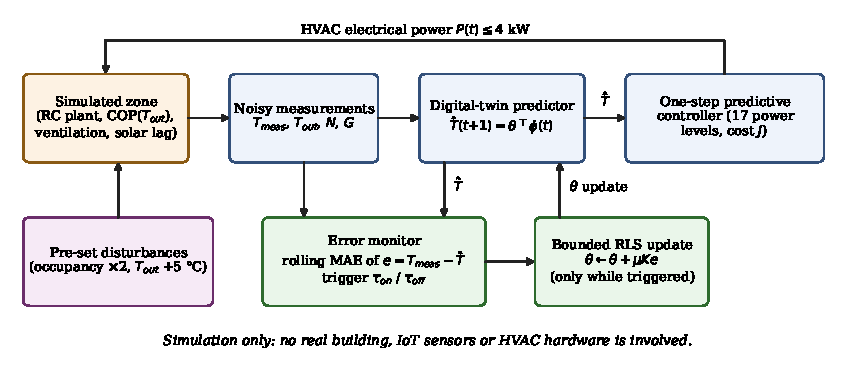
\includegraphics[width=0.82\textwidth]{fig01_architecture.pdf}
\caption{Architecture of the simulated adaptive digital-twin loop. All blocks are software; no real building, IoT sensor or HVAC equipment is involved.}
\label{fig:arch}
\end{figure*}

\subsection{Simulated zone (the ``true'' building)}\label{sec:plant}
The zone is a single classroom-like space modelled as one thermal capacitance. Let $T$ be the indoor temperature (\degC), $T_{out}$ the outdoor temperature (\degC), $N$ the number of occupants, $G$ the solar irradiance (W/m$^2$), and $P$ the HVAC electrical power (kW). The heat balance is
\begin{multline}
C\,\frac{dT}{dt}=(U_a+k_vN)(T_{out}-T)+q_pN+q_e\,u_{occ}\\
+Q_s+w-1000\,\mathrm{COP}(T_{out})\,P,
\label{eq:plant}
\end{multline}
\begin{equation}
\tau_s\frac{dQ_s}{dt}=A_sG-Q_s,
\label{eq:solar}
\end{equation}
\begin{equation}
\mathrm{COP}(T_{out})=\mathrm{clip}\big[3.5-0.06(T_{out}-27),\,2,\,4\big].
\label{eq:cop}
\end{equation}
Every term of \eqref{eq:plant} is a power in watts: $C$ is in J/K and $dT/dt$ in K/s; $U_a$ and $k_v$ are in W/K (the latter per occupant, representing demand-controlled ventilation); $q_p$ and $q_e$ are in W; $u_{occ}\in\{0,1\}$ marks occupied steps; $w$ is zero-mean process noise in W; and the factor 1000 converts kW to W. The cooling term uses a COP that falls as outdoor temperature rises. The model is integrated with 60\,s sub-steps, inputs held constant over each 15-minute step. Table~\ref{tab:params} lists all values. They are assumed, not measured, and no claim is made that they represent a particular building.

\begin{table}[!t]
\renewcommand{\arraystretch}{1.05}
\caption{Assumed simulation parameters (not calibrated to a real building)}
\label{tab:params}
\centering\footnotesize
\begin{tabular}{lll}
\hline
Symbol & Meaning & Value\\
\hline
$C$ & Thermal capacitance & $5.0\times10^{6}$ J/K\\
$U_a$ & Envelope conductance & 150 W/K\\
$k_v$ & Ventilation conductance & 3.0 W/K per person\\
$q_p$ & Sensible gain per person & 75 W\\
$q_e$ & Equipment gain (occupied) & 400 W\\
$A_s$, $\tau_s$ & Solar aperture, lag & 2.5 m$^2$, 1800 s\\
$\sigma_w$ & Process-noise std.\ dev. & 150 W\\
$\sigma_v$ & Sensor-noise std.\ dev. & 0.1 \degC\\
$P_{max}$ & Power limit, resolution & 4.0 kW, 0.25 kW\\
-- & Cooling schedule & 07:00--18:00\\
-- & Peak occupancy & 30 people\\
-- & Evaluation comfort band & 22--26 \degC\\
-- & Control band (all controllers) & 23--25 \degC\\
\hline
\end{tabular}
\end{table}

Three features make the plant deliberately different from the predictor's structure: the occupant-dependent ventilation term couples $N$ and $T_{out}-T$ multiplicatively, the COP depends on $T_{out}$, and solar gain is lagged. Without such mismatch, a linear predictor fitted to the plant would be nearly exact and the adaptation question would be empty.

\subsection{ARX predictor}\label{sec:arx}
The digital twin predicts the next temperature from quantities available at time $t$:
\begin{equation}
\that(t{+}1)=\boldsymbol{\theta}^{\top}\boldsymbol{\phi}(t),
\label{eq:arx}
\end{equation}
\begin{equation}
\boldsymbol{\phi}=[\,T_{m},\,T_{out},\,N/10,\,G/1000,\,P,\,1\,]^{\top},
\end{equation}
where $T_m=T+v$ is the measured temperature and $\boldsymbol{\theta}=[a,b,c,d,e,f]^{\top}$. Under an Euler discretisation of \eqref{eq:plant} with $\Delta t=900$\,s and nominal $N=30$, one expects $a\approx0.957$, $b\approx0.043$ and $e\approx-0.56$\,\degC/kW, so the coefficients have a physical reading and can be inspected. The model is fitted by least squares to the three-day initialisation record (288 samples), giving mean estimates $a=\ThetaInitA$, $b=\ThetaInitB$, $c=\ThetaInitC$, $d=\ThetaInitD$, $e=\ThetaInitE$ and $f=\ThetaInitF$ across seeds. The in-sample residual MAE, \MaeRef\,\degC, is the reference noise level used later for the trigger threshold. The initialisation record is produced by the thermostat with random power perturbations on 25\% of cooling steps, which supplies the excitation needed to identify the effect of $P$.

\subsection{Controllers}\label{sec:controllers}
\emph{Thermostat.} A two-stage hysteresis rule with setpoint 24\,\degC\ and deadband $\pm1$\,\degC: cooling starts at 25\,\degC\ and stops at 23\,\degC; while on, it uses 2\,kW, or 4\,kW once $T_m\ge25.5$\,\degC. It sees only $T_m$.

\emph{Predictive controller (shared by the three AI variants).} At each step the controller evaluates \eqref{eq:arx} for each of 17 power levels $\mathcal{L}=\{0,0.25,\dots,4\}$\,kW and picks
\begin{equation}
P^{*}=\arg\min_{P\in\mathcal{L}}\; w_c\big[(\that-25)_+^{2}+(23-\that)_+^{2}\big]+\lambda_e P,
\label{eq:cost}
\end{equation}
with $w_c=20$\,\degC$^{-2}$ and $\lambda_e=0.3$\,kW$^{-1}$, fixed before any simulation. Horizon is one step, and the controller uses current values of $T_m$, $T_{out}$, $N$ and $G$ with no forecast.

\emph{Fixed AI.} $\boldsymbol{\theta}$ stays at its initial value.

\emph{Gated ADT.} After each new measurement the error $e(t{+}1)=T_m(t{+}1)-\that(t{+}1)$ is computed, and the rolling mean absolute error $\bar e$ over $W=8$ steps (two hours) is compared with thresholds: updating starts when $\bar e>\tau_{on}=\kappa\cdot\mathrm{MAE}_{ref}$ with $\kappa=\TauOn$ and stops when $\bar e<\TauOff\,\tau_{on}$. While active, a bounded RLS step is applied,
\begin{align}
\mathbf{K}&=\frac{\mathbf{P}\boldsymbol{\phi}}{\lambda_f+\boldsymbol{\phi}^{\top}\mathbf{P}\boldsymbol{\phi}},\quad
\boldsymbol{\theta}\leftarrow\boldsymbol{\theta}+\mu\,\mathbf{K}\,\tilde e,\label{eq:rls1}\\
\mathbf{P}&\leftarrow\frac{1}{\lambda_f}\big(\mathbf{P}-\mathbf{K}\boldsymbol{\phi}^{\top}\mathbf{P}\big),\label{eq:rls2}
\end{align}
where $\tilde e$ is $e$ clipped to $\pm1$\,\degC, $\lambda_f=\LamF$ is the forgetting factor and $\mu=\MuLR$ is the learning rate. Three further protections apply: parameters are clipped to wide physical bounds, the covariance trace is capped at 20 times its initial value, and the update is conditional on the trigger. $\mathbf{P}$ starts from the inverse data matrix of the initialisation fit, scaled so that its information equals that of the forgetting window. Only the measurement at $t{+}1$ and the regressor from $t$ enter the update, so no future data are used.

\emph{Always-on RLS.} The same update \eqref{eq:rls1}--\eqref{eq:rls2}, applied at every step. This ablation separates the effect of adapting from the effect of gating.

\subsection{Performance metrics}
With $\Delta t=0.25$\,h, the energy over $K=96$ steps is
\begin{equation}
E=\sum_{k=1}^{K}P(k)\,\Delta t\quad[\mathrm{kWh}].
\label{eq:energy}
\end{equation}
For a band $[T_{lo},T_{hi}]$ the violation at time $t$ is $v(t)=\max(0,T-T_{hi})+\max(0,T_{lo}-T)$ in \degC, zero inside the band, and the mean violation is
\begin{equation}
\bar V=\frac{1}{|\mathcal{O}|}\sum_{t\in\mathcal{O}}v(t),
\label{eq:viol}
\end{equation}
where $\mathcal{O}$ is the set of occupied steps and $T$ is the true simulated temperature. This is computed for the evaluation band 22--26\,\degC\ and for the narrower 23--25\,\degC\ control band, the latter a secondary metric defined before the experiment. Prediction accuracy is
\begin{equation}
\mathrm{MAE}=\frac{1}{K}\sum_{k=1}^{K}\big|T(k{+}1)-\that(k{+}1)\big|,
\label{eq:mae}
\end{equation}
where $T$ is the noise-free simulated temperature and $\that$ is the prediction made one step earlier. Peak power is $\max_k P(k)$. Controller compute time is measured with a wall-clock timer.

%--------------------------------------------------------------------
\section{Simulation Methodology}
\subsection{Timeline and exogenous signals}
The step is 15 minutes. Each seed produces three initialisation days followed by one 24-hour evaluation day, all starting from the same plant state for every controller. Outdoor temperature follows $T_{out}=29+\delta_d+5\sin[2\pi(h-9)/24]$ plus an AR(1) term ($\phi=0.9$, innovation std.\ 0.15\,\degC), with a daily offset $\delta_d\sim\mathcal{N}(0,1)$\,\degC. Irradiance is a half-sine between 06:00 and 18:00 with peak 850\,W/m$^2$, multiplied by an AR(1) cloud factor with mean 0.85. Occupancy rises from one third of its peak to 30 people between 08:00 and 09:00, halves from 13:00 to 14:00, and falls off between 17:00 and 18:00, scaled by a daily factor $\mathcal{N}(1,0.05^2)$. Fig.~\ref{fig:inputs} shows one seed.

\begin{figure}[!t]
\centering
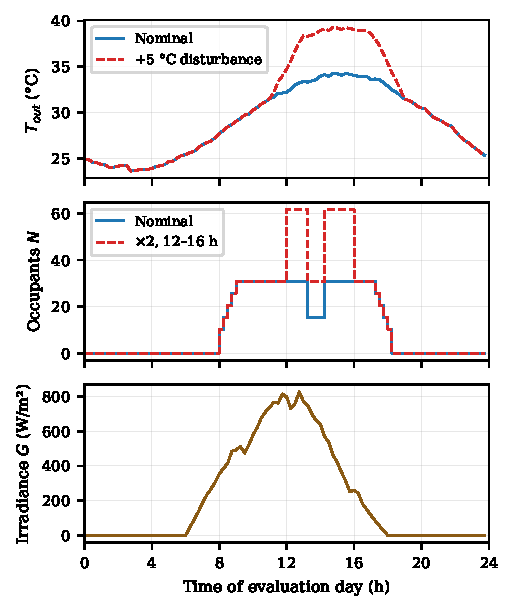
\includegraphics[width=\columnwidth]{fig02_inputs.pdf}
\caption{Outdoor temperature, occupancy and solar irradiance on the evaluation day for seed 0, nominal and with the combined disturbance.}
\label{fig:inputs}
\end{figure}

\subsection{Scenarios}
The disturbances were fixed before the experiment and applied to the evaluation day only (Table~\ref{tab:scen}). The ``window'' is the period over which period-specific MAE is reported.

\begin{table}[!t]
\renewcommand{\arraystretch}{1.05}
\caption{Pre-specified evaluation scenarios}
\label{tab:scen}
\centering\footnotesize
\begin{tabular}{lp{0.24\columnwidth}p{0.32\columnwidth}l}
\hline
Scenario & Occupancy & Outdoor temperature & Window (h)\\
\hline
Baseline & Nominal & Nominal & 11--19\\
Occupancy & $\times2$, 12:00--16:00 & Nominal & 12--16\\
Outdoor & Nominal & Ramp 0 to $+5$\,\degC\ over 11--13\,h, hold to 17\,h, ramp to 0 by 19\,h & 11--19\\
Combined & As occupancy & As outdoor & 11--19\\
\hline
\end{tabular}
\end{table}

\subsection{Seeds, fairness and information}
Evaluation used seeds 0--19. Within a seed, weather, occupancy, process noise and sensor noise are generated once and shared by every controller and scenario (common random numbers), so differences between controllers are not caused by different noise. The three AI controllers share the same initial parameters, cost weights, power levels and measurements. They differ only in the update rule. The thermostat has less information than the AI controllers, since it sees only $T_m$ and not $T_{out}$, $N$ or $G$, and its 15-minute sampling is coarse; this asymmetry is discussed with the results. Because the AI controllers drive different trajectories, a second comparison runs all three predictors passively alongside the thermostat on the \emph{same} trajectory, which isolates predictor quality from control effects.

\subsection{Hyper-parameter selection and verification}
The update hyper-parameters ($\kappa$, $\lambda_f$, $\mu$ for the gated arm; $\lambda_f$, $\mu$ for the always-on arm) were chosen on a separate set of ten development seeds (1000--1009) from equal-sized grids, using closed-loop MAE as the criterion; the evaluation seeds were not used for this. The initial settings were $\kappa=2$, $\lambda_f=0.98$, $\mu=0.5$; only $\kappa$ changed (to \TauOn), and that value is the smallest in its grid, so it may not be the optimum. Seventeen automated tests check the plant against its analytic response, steady state and energy bookkeeping, the metric definitions, the thermostat logic, RLS convergence and bounds, reproducibility, and absence of future-data leakage (changing inputs after step $k^{*}$ left all decisions and predictions up to $k^{*}$ unchanged for every controller). Parameter bounds were never reached in any evaluation run.

%--------------------------------------------------------------------
\section{Results and Discussion}
All values below come from the executed simulation (320 closed-loop runs and 240 passive-predictor runs). Table~\ref{tab:summary} gives the main outcomes and Table~\ref{tab:paired} the paired differences. Measured results and our interpretations are kept apart.

\input{tables/tab_summary.tex}

\begin{figure*}[!t]
\centering
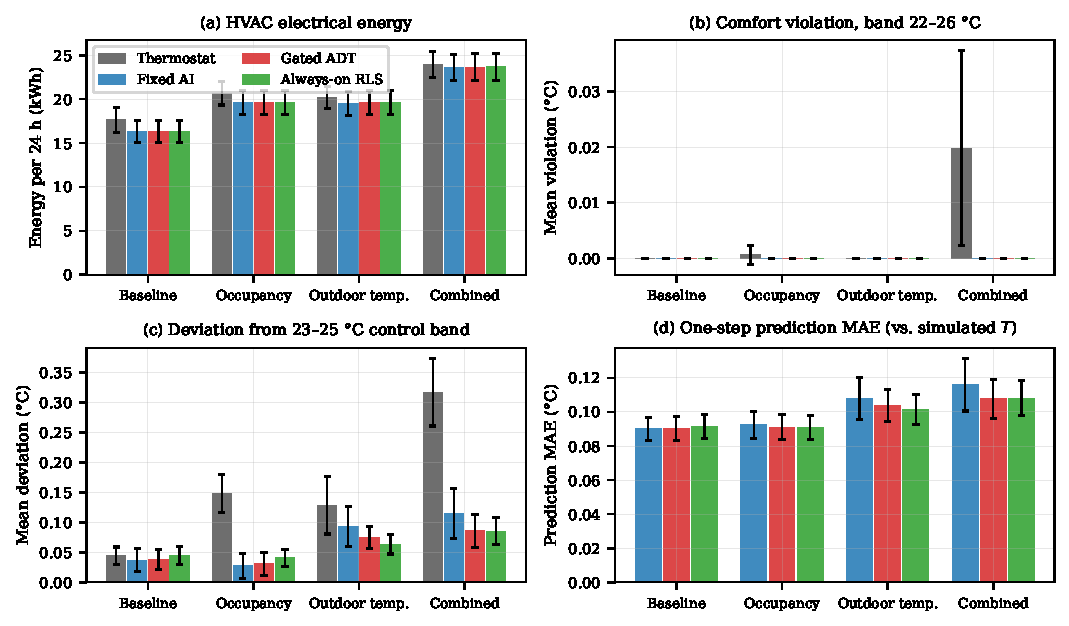
\includegraphics[width=0.85\textwidth]{fig07_summary_bars.pdf}
\caption{Scenario comparison over 20 seeds (mean, error bars one standard deviation): (a) energy, (b) violation of the 22--26\,\degC\ band, (c) deviation from the 23--25\,\degC\ band, (d) prediction MAE.}
\label{fig:bars}
\end{figure*}

\begin{figure*}[!t]
\centering
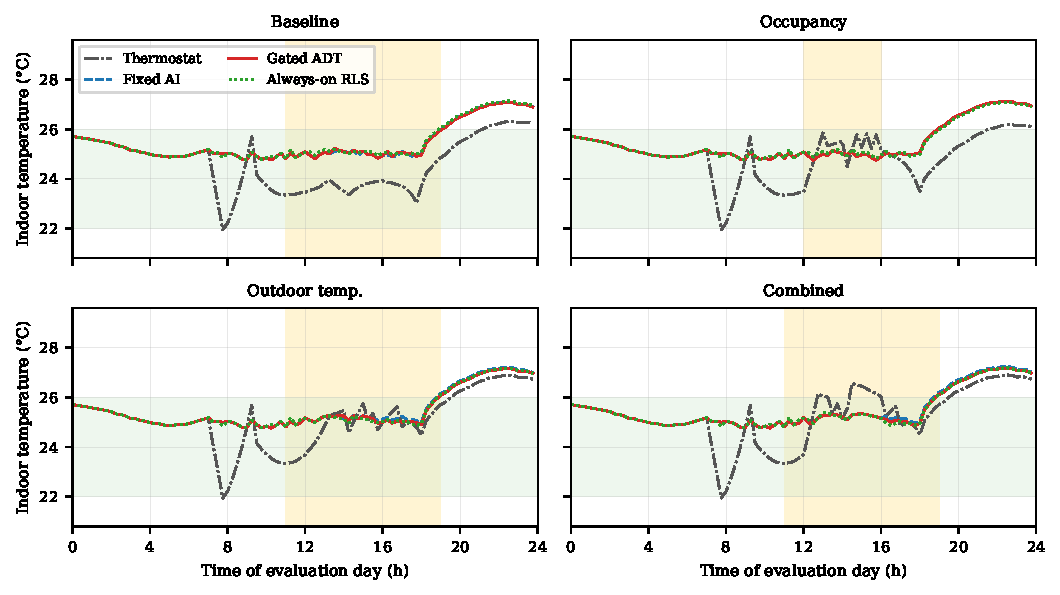
\includegraphics[width=0.92\textwidth]{fig03_indoor_temperature.pdf}
\caption{Simulated indoor temperature for all controllers in the four scenarios (seed 0). Green: 22--26\,\degC\ evaluation band; yellow: disturbance window. Comfort is scored only while the room is occupied (08:00--18:00).}
\label{fig:temp}
\end{figure*}

\subsection{Energy}
\emph{Measured.} The AI controllers used less energy than the thermostat in every scenario: the fixed AI controller changed energy by \PctEnergyFxThBase\%, \PctEnergyFxThOcc\%, \PctEnergyFxThOut\% and \PctEnergyFxThComb\% relative to it in the baseline, occupancy, outdoor and combined cases. Among the AI variants the spread was small. In the combined case the energies were \EnergyCombFx, \EnergyCombGt\ and \EnergyCombAl\,kWh (fixed, gated, always-on). Relative to the fixed predictor, gated adaptation changed energy by \DEnergyOutGtFx\,kWh in the outdoor case ($p\,\PEnergyOutGtFx$) and by \DEnergyCombGtFx\,kWh in the combined case ($p\,\PEnergyCombGtFx$); in the baseline case the difference was \DEnergyBaseGtFx\,kWh.

\emph{Interpretation.} The saving relative to the thermostat should not be credited to learning. The thermostat's 2\,kW first stage removes roughly one degree per step under light load, so at 15-minute sampling it overshoots below its 23\,\degC\ switch-off point and then holds the room cooler than necessary (Fig.~\ref{fig:temp}), whereas the predictive controller modulates power finely and operates near the edge of the control band. A better-tuned or finer-sampled thermostat would narrow this gap. Adaptation itself changed energy by at most about 0.5\%.

\subsection{Comfort}
\emph{Measured.} Against the 22--26\,\degC\ evaluation band, none of the 240 AI-controller runs had any violation. The thermostat produced violations in all 20 combined runs (mean \ViolCombTh\,\degC, mean per-run maximum \VMaxCombTh\,\degC) and in 5 of 20 occupancy runs (mean \ViolOccTh\,\degC), and none otherwise. This band therefore separates the thermostat from the AI controllers but not the AI controllers from each other. The tighter 23--25\,\degC\ control band does. There, the mean deviation of the fixed, gated and always-on variants was respectively \TightOutFx, \TightOutGt\ and \TightOutAl\,\degC\ in the outdoor case and \TightCombFx, \TightCombGt\ and \TightCombAl\,\degC\ in the combined case. Relative to the fixed predictor, gating changed the deviation by \PctTightGtFxOut\% and \PctTightGtFxComb\% in those two cases. In the baseline and occupancy cases, however, gating did not help (\PctTightGtFxBase\% and \PctTightGtFxOcc\%) and always-on updating worsened it (\PctTightAlFxBase\% and \PctTightAlFxOcc\%).

\emph{Interpretation.} The direction of the comfort gain matches the energy increase above: adapted predictions lead to somewhat more cooling when it is needed. Fig.~\ref{fig:power} shows that in the combined case the 4\,kW limit is reached for several hours, so the controllers are partly capacity-limited and cannot differ greatly.

\begin{figure}[!t]
\centering
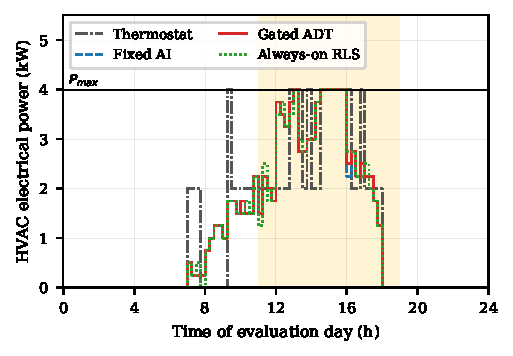
\includegraphics[width=\columnwidth]{fig06_hvac_power.pdf}
\caption{HVAC electrical power in the combined scenario (seed 0).}
\label{fig:power}
\end{figure}

\subsection{Prediction accuracy and response to disturbances}
\emph{Measured.} Closed-loop MAE of the fixed predictor rose from \MaeBaseFx\,\degC\ in the baseline to \MaeOutFx\,\degC\ (outdoor) and \MaeCombFx\,\degC\ (combined), while doubled occupancy alone had little effect (\MaeOccFx\,\degC). Gating lowered MAE to \MaeOutGt\,\degC\ and \MaeCombGt\,\degC\ in those two cases, and always-on RLS to \MaeOutAl\,\degC\ and \MaeCombAl\,\degC. For gating, the paired difference to the fixed predictor was \DMaeOutGtFx\,\degC\ (outdoor) and \DMaeCombGtFx\,\degC\ (combined), better in \WMaeOutGtFx\ and \WMaeCombGtFx\ of 20 seeds respectively. Inside the disturbance window the effect is larger (Table~\ref{tab:shadow} and Fig.~\ref{fig:err}): on the common trajectory the fixed predictor's MAE in the window was \ShMaeDurOutFx\,\degC\ (outdoor) and \ShMaeDurCombFx\,\degC\ (combined), against \ShMaeDurOutGt\ and \ShMaeDurCombGt\,\degC\ for gating. Before the window all predictors were equal at the sensor-noise floor of roughly 0.09--0.10\,\degC. In the baseline and occupancy scenarios, gating gave no reliable change in overall MAE (\DMaeBaseGtFx\ and \DMaeOccGtFx\,\degC).

\begin{figure}[!t]
\centering
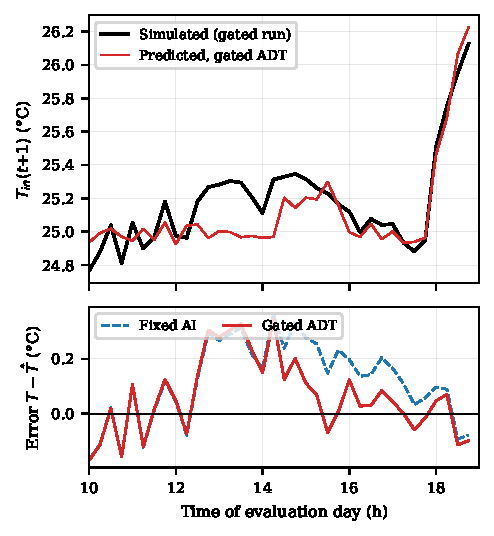
\includegraphics[width=\columnwidth]{fig04_pred_vs_sim.pdf}
\caption{Predicted versus simulated next-step temperature in the combined scenario (seed 0): (top) simulated and gated-ADT predicted temperature; (bottom) prediction error of the fixed and gated predictors.}
\label{fig:pred}
\end{figure}

\input{tables/tab_shadow.tex}

\begin{figure}[!t]
\centering
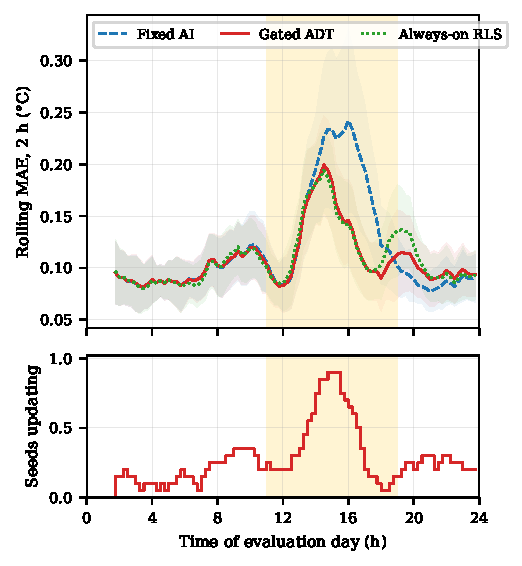
\includegraphics[width=\columnwidth]{fig05_prediction_error.pdf}
\caption{Combined scenario, passive predictors on the common thermostat trajectory, 20 seeds: (top) two-hour rolling MAE (mean $\pm$ one standard deviation); (bottom) share of seeds in which the gated predictor is updating.}
\label{fig:err}
\end{figure}

\emph{Speed of response.} The gated predictor reacted slowly. Averaged over seeds that updated at all, the first update after the window opened came \ShDelayOut\ minutes later in the outdoor case and \ShDelayComb\ minutes later in the combined case, and updates were active in up to roughly 90\% of seeds around 15:00 (Fig.~\ref{fig:err}). Part of this lag is inherent, since the temperature ramp is gradual and the monitor needs two hours of data. The trigger was also not clean: before the window opened it fired in about \ShFalseBase\% of baseline steps, a false-alarm rate set by $\kappa=\TauOn$ relative to a noise level that already contains sensor noise. Updates were active in \UpdBaseGt\% of baseline steps and \UpdCombGt\% of combined steps, against 100\% for the always-on variant.

\subsection{Gating versus always-on updating}
Always-on RLS reached slightly lower MAE than gating in the outdoor case (\MaeOutAl\ versus \MaeOutGt\,\degC) and a lower control-band deviation (\TightOutAl\ versus \TightOutGt\,\degC), at a higher energy of \EnergyOutAl\ versus \EnergyOutGt\,kWh. In the combined case the two were indistinguishable on MAE and deviation. In the baseline and occupancy cases always-on updating was worse than gating on control-band deviation (Table~\ref{tab:paired}). Fig.~\ref{fig:params} shows the parameter movements: they are small, and the always-on estimate of the cooling coefficient $e$ shifts further and more abruptly than the gated one. We did not isolate the cause. Gating therefore trades a little responsiveness for avoiding unnecessary updates; it did not dominate always-on updating on every metric.

\input{tables/tab_paired.tex}

\begin{figure}[!t]
\centering
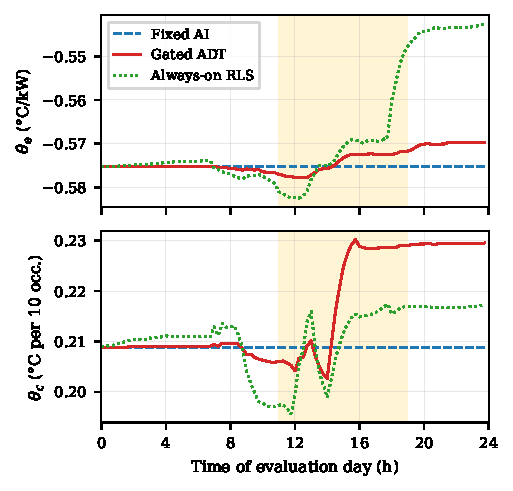
\includegraphics[width=\columnwidth]{fig08_parameter_evolution.pdf}
\caption{Mean parameter trajectories over 20 seeds in the combined scenario: cooling coefficient $\theta_e$ (top) and occupancy coefficient $\theta_c$ (bottom).}
\label{fig:params}
\end{figure}


\subsection{Cost, consistency and possible explanations}
Controller computation per simulated day was \TimeBaseFx\,ms for the fixed predictor and \TimeBaseGt\,ms for the gated one, so the extra cost of adapting is negligible at this scale; absolute timings depend on the machine. Results were consistent across seeds for the outdoor and combined cases (Table~\ref{tab:paired}) but not for the baseline and occupancy cases. The paired tests are exploratory: \NTests\ comparisons were computed, and only those marked $\dagger$ survive a Bonferroni correction.

\emph{Hypotheses (not tested directly).} The outdoor disturbance pushes the plant outside the conditions seen during initialisation, where the assumed COP decline makes the fixed predictor overestimate cooling; adaptation corrects part of this. Doubling occupancy changes a term the linear model represents reasonably, so there is less to correct, and the small occupancy-window gain is not reliable. These explanations are consistent with the data but would need targeted experiments, such as varying the COP slope, to confirm.

\emph{Practical significance.} The largest reduction in MAE is under 0.01\,\degC\ overall and about 0.03\,\degC\ inside the window, against 0.1\,\degC\ of sensor noise and a 4\,\degC\ comfort band. The effects are statistically consistent but physically small in this setting. The claim supported is limited: in this synthetic zone, gated adaptation improved prediction and control-band adherence under the temperature-related disturbances, at a small energy cost, and did nothing useful otherwise.

%--------------------------------------------------------------------
\section{Limitations and Future Work}
The conclusions are bounded by the following.
\begin{itemize}
\item The thermal model is a one-capacitance simplification; its parameters, including the COP slope, are assumed, and results depend on them.
\item Nothing was calibrated against, or compared with, measurements from a real building.
\item Only one weather shape, one occupancy schedule and four disturbances were tested, over 20 seeds.
\item Hyper-parameters were tuned on development seeds, and the selected threshold factor lies at the edge of its grid.
\item The thermostat is a coarse reference with less information than the AI controllers; the energy gap to it should not be generalised. No tuned MPC was compared.
\item There was no IoT integration, hardware-in-the-loop testing or evidence about commercial buildings.
\item The literature review rests on nine verified sources, mostly read at abstract level, and does not constitute a systematic review.
\end{itemize}
Natural next steps, none of which has been performed here, are coupling the controller to EnergyPlus or a calibrated building model, testing against measured data, combining gating with adaptive MPC and uncertainty estimates, and sweeping the severity and type of disturbance to find where adaptation starts to pay off.

%--------------------------------------------------------------------
\section{Conclusion}
A simulation-only adaptive digital twin was compared with a frozen predictor, an always-on update and a thermostat in a single cooled zone. Prediction-error-gated updating reduced prediction error and control-band deviation under outdoor-temperature and combined disturbances, used a few tenths of a percent more energy, and was not beneficial in the baseline or occupancy-only cases. Always-on updating was slightly better under outdoor stress but slightly worse without it. The improvements are consistent across seeds but small in absolute terms, and they apply to a synthetic, uncalibrated plant. The released code and configuration allow every figure and table here to be regenerated and the assumptions to be varied.

\section*{Data, Code and AI-Assistance Disclosure}
Code, configuration and result files: [repository or archive link to be added]. This manuscript, the simulation code and the analysis scripts were prepared with the assistance of an AI model (Claude, Anthropic). The authors remain responsible for checking all content, and this statement should be adapted to the disclosure policy of the institution and venue. [Authors to complete.]

\begin{thebibliography}{10}
\bibitem{ibrahim2026} N. I. Ibrahim, C. Vering, N. Giannetti, M. Kim, Sholahudin, T. Storek, D. M\"uller, and K. Saito, ``State-of-the-art of the digital twin concept in HVAC+R systems for thermal management of buildings,'' \emph{Renew. Sustain. Energy Rev.}, vol.~229, Art. no.~116601, 2026, doi: 10.1016/j.rser.2025.116601.
\bibitem{hodavand2023} F. Hodavand, I. J. Ramaji, and N. Sadeghi, ``Digital twin for fault detection and diagnosis of building operations: A systematic review,'' \emph{Buildings}, vol.~13, no.~6, p.~1426, 2023, doi: 10.3390/buildings13061426.
\bibitem{drgona2020} J. Drgo\v{n}a \emph{et al.}, ``All you need to know about model predictive control for buildings,'' \emph{Annu. Rev. Control}, vol.~50, 2020, doi: 10.1016/j.arcontrol.2020.09.001.
\bibitem{wang2020} Z. Wang and T. Hong, ``Reinforcement learning for building controls: The opportunities and challenges,'' \emph{Appl. Energy}, vol.~269, 2020, doi: 10.1016/j.apenergy.2020.115036.
\bibitem{zeng2021} T. Zeng and P. Barooah, ``An adaptive MPC scheme for energy-efficient control of building HVAC systems,'' arXiv:2102.03856, 2021.
\bibitem{eini2019} R. Eini and S. Abdelwahed, ``Learning-based model predictive control for smart building thermal management,'' arXiv:1909.05331, 2019.
\bibitem{burger2017} E. M. Burger and S. J. Moura, ``ARX model of a residential heating system with backpropagation parameter estimation algorithm,'' in \emph{Proc. ASME Dyn. Syst. Control Conf.}, 2017, doi: 10.1115/DSCC2017-5315.
\bibitem{guo2025} S. Guo, Z. Wei, H. Wu, H. Fang, and X. Zhai, ``Real-time prediction of thermal load and indoor temperature for buildings with a recursive identification method in noise conditions,'' \emph{Energy}, vol.~335, 2025, doi: 10.1016/j.energy.2025.138022.
\bibitem{ashrae55} \emph{Thermal Environmental Conditions for Human Occupancy}, ANSI/ASHRAE Standard 55-2023, 2023.
\end{thebibliography}

\end{document}
